\documentclass[12pt,a4paper]{article}
\usepackage[utf8]{inputenc}
\usepackage[brazilian]{babel}
\usepackage{indentfirst}
\usepackage{pdfpages}

\setlength{\parskip}{0.5em}
\renewcommand{\baselinestretch}{1.1}

\title{Sistema Web para Instalação de ERBs}
\author{Mateus Nakajo de Mendonça  \\
	Eric Rodrigues Pires  \\
	\em{Orientador: Bruno de Carvalho Albertini}
	}

\date{19 de fevereiro de 2018}

\begin{document}
\maketitle

\begin{abstract}
Este projeto de formatura tem como objetivo criar um sistema capaz de calcular
posições para a instalação de Estações Radiobase (ERBs) de forma que a área
coberta pela rede de ERBs seja máxima. A partir da região dada como entrada, o
sistema obterá seus dados geográficos através de um software SIG e utilizará
programação linear para a otimização da posição de instalação. Para interface
com o usuário do sistema, criaremos uma aplicação Web responsiva que permita
selecionar a região na qual se pretende instalar uma ERB e mostra as posições
ideais para instalação.
\end{abstract}

\section{Introdução}
Na revolução da informação em que vivemos hoje, em que cada vez mais pessoas
estão conectadas à rede, o acesso à Internet tem se tornado cada vez mais
essencial no dia-a-dia, até mesmo a populações consideradas isoladas. Empresas
bem conhecidas, como Vivo e Claro, vêm se empenhando para garantir melhor
acesso a mais pessoas, mas se deparam com problemas de engenharia nesta
tarefa.

A extensão territorial e a densidade demográfica desigual do Brasil são dois
dentre vários fatores que tornam problemas de telecomunicação mais complexos.
A dimensão deste problema gera um grande potencial de mercado para empresas
terceirizadas, voltadas à instalação de Estações Radiobase (ERBs) para
compartilhamento ou aluguel de células telefônicas às grandes empresas de
telecomunicação. Dessa forma, há demanda do mercado por ferramentas que
simplifiquem e/ou automatizem a tarefa de estudo de localização de ERBs.

\section{Objetivo}
O objetivo deste projeto de formatura é criar um sistema que permita calcular
posições para a instalação de antenas de telefonia de forma a maximizar o
alcance delas. Com esse fim, levaremos em conta dados geográficos para
realizarmos os cálculos.

Também é de grande importância que tal sistema tenha uma interface prática
para os usuários. Portanto, uma interface web que apresente os dados
requisitados é essencial para o projeto.

Outras possíveis ramificações do projeto para showcase ao público geral, que não
é o público-alvo, é a localização de antenas a partir do próprio celular do
usuário, e a estimativa de posição do dispositivo pelas antenas encontradas.

\subsection{Sistema de Informação Geográfica}
SIG (Sistema de Informação Geográfica) é um sistema computacional capaz de
obter, gravar, gerir, analisar e visualizar dados geográficos. Seu uso permite
tomar decisões, analisar estatísticas e resolver problemas de otimização a
partir de dados geográficos. O SIG pode ser usado tanto em lojas de varejo para
decidir onde abrir uma nova filial, como em rastrear padrões de migração,
controle e o monitoramento do desmatamento, planejamento urbano, etc.

No nosso projeto, usaremos um software SIG para gravar e exibir a posição de
ERBs (Estações Radiobase) atuais, o relevo e os consumidores atingidos pela
rede de ERBs. Com essas informações, determinaremos as posições ótimas de
ERBs de modo a maximizar a área de cobertura do sistema de telefonia.
Para tanto, aplicaremos técnicas de programação linear, uma vez que
estamos diante de um problema de otimização cuja função a ser otimizada
é linear em relação às variáveis de entrada.

O SIG utilizado será integrado à plataforma web Django, pelo módulo GeoDjango,
que utiliza como banco de dados o PostGIS (baseado em Postgres). Serão armazenados
dados públicos de localização de ERBs, relevo e densidade populacional. Ele
será também responsável pelos cálculos realizados para a localização de novas
antenas.

\subsection{Interface Web}
Para interação com o usuário, criaremos um front-end de uma aplicação Web que
permita selecionar a região na qual se pretende instalar alguma ERB.
Esta interface se comunicará com o back-end do SIG, para obter e calcular os
dados desejados.

O design deverá ser responsivo, podendo ser utilizado em plataformas mobile
ou desktop, e simples, com opções simples para apenas verificar a posição ótima
de instalação de antenas em determinada área escolhida pelo usuário. Para isso,
a interface deverá exibir um mapa, como por exemplo o da plataforma
OpenStreetMap, com as informações do SIG, que permita ao usuário selecionar uma
área desejada. Os dados serão calculados no back-end e exibidos ao usuário na
tela. Para isso, será necessário desenvolver um front-end possivelmente
dinâmico.

No projeto, para facilidade de desenvolvimento, utilizaremos o framework Django,
escrito em Python. A integração de single-page com o back-end deverá ser feita
com o módulo de API REST do Django.

\section{Desenvolvimento}

Para iniciar o desenvolvimento, definimos a árvore de pré-requisitos da
Figura~\ref{fig:prerequisitos}. Decidimos priorizar o back-end com o SIG e
deixar a interface web em segundo plano; porém, para o desenvolvimento de ambos,
necessitaremos do Django com a extensão GeoDjango e banco PostGIS.

\begin{figure*}[htp]
    \centering
    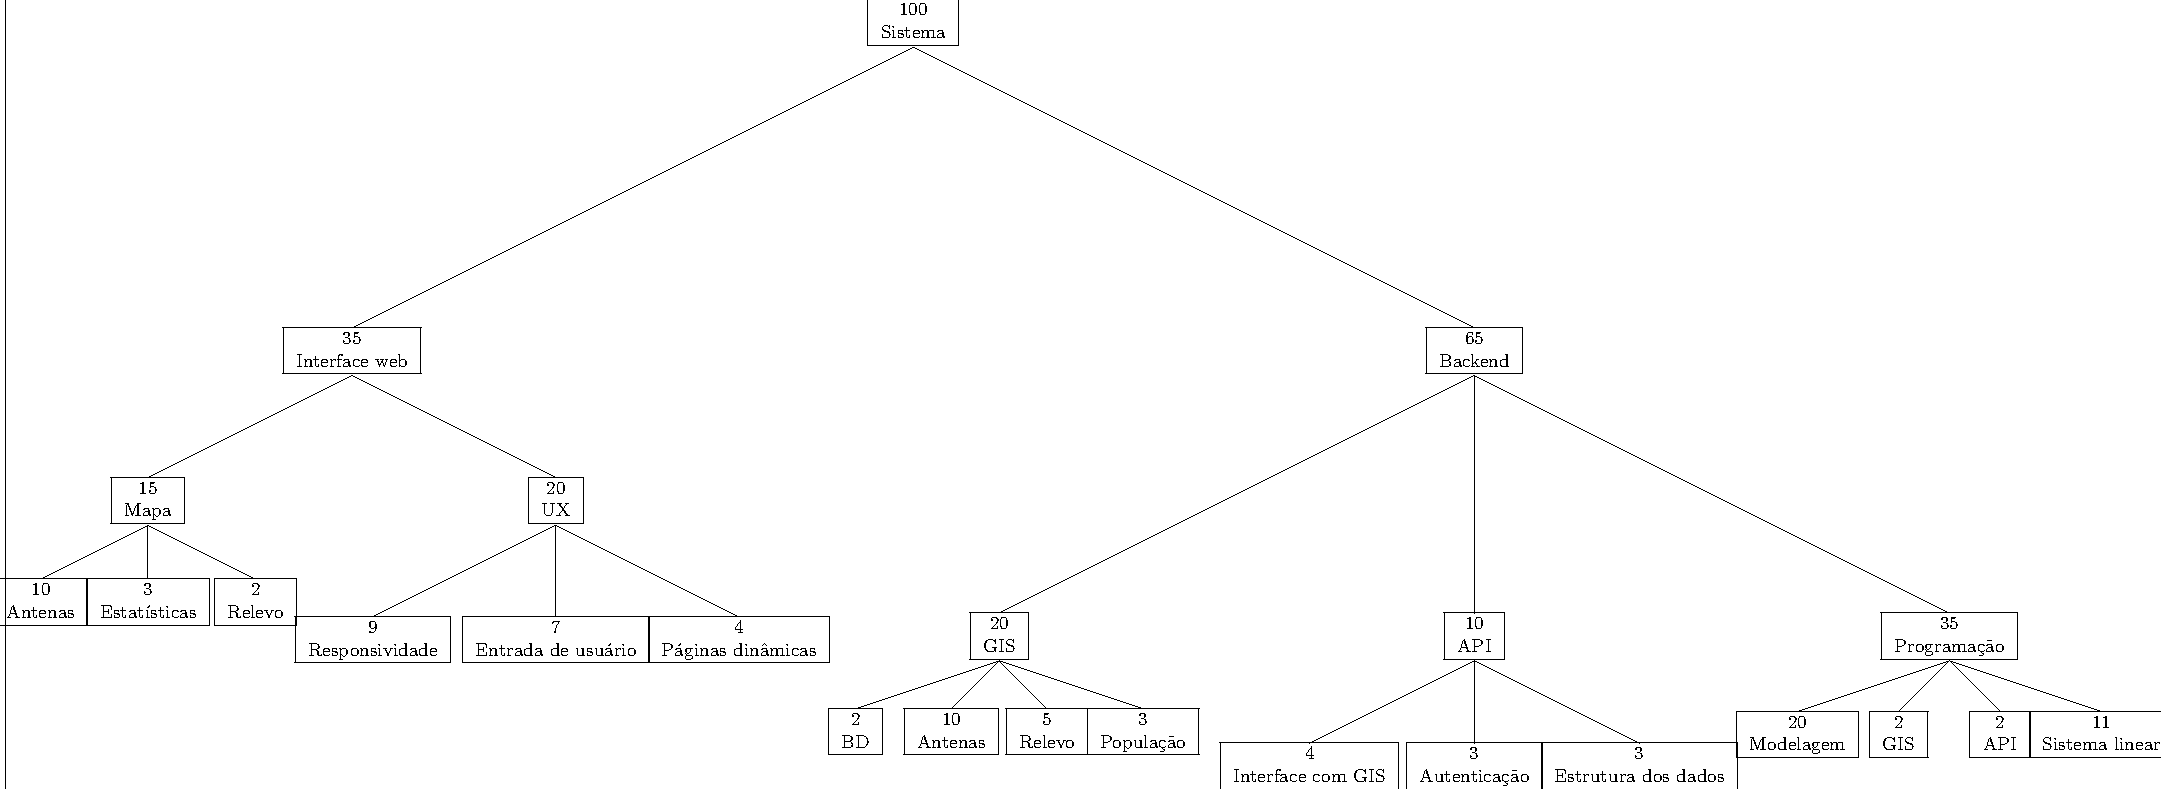
\includegraphics[width=1.4\textwidth, angle=270]{../misc/arvore_prerequisitos.pdf}
	\caption{Árvore de pré-requisitos}
	\label{fig:prerequisitos}
\end{figure*}

Depois, buscamos os dados necessários. As informações públicas de ERBs no Brasil
foram encontrados em \cite{mapa-erb}, no formato CSV. Além disso, encontramos
mapas de Relevo e Densidade Populacional em \cite{mapa-ibge}. Esses dados serão
importados ao nosso GIS.

\begin{thebibliography}{9}

\bibitem{mapa-erb}
Telebrasil.
\textit{Mapa de ERBs Brasil (antenas)}.
Disponível em: http://www.telebrasil.org.br/panorama-do-setor/mapa-de-erbs-antenas.
Acesso em: 31 de janeiro de 2018.

\bibitem{mapa-ibge}
Instituto Brasileiro de Geografia e Estatística.
\textit{WMS do ArcGIS}.
Disponível em: https://mapas.ibge.gov.br/interativos/servicos/wms-do-arcgis.html.
Acesso em: 10 de fevereiro de 2018.

\end{thebibliography}

\end{document}


